% This is samplepaper.tex, a sample chapter demonstrating the
% LLNCS macro package for Springer Computer Science proceedings;
% Version 2.20 of 2017/10/04
%
\documentclass[runningheads]{llncs}
%
\usepackage{graphicx}
\newcommand{\SWAT}{SWAF}
\usepackage{graphicx}
\usepackage{listings}
\usepackage{subfig}
\usepackage[utf8]{inputenc}
\graphicspath{ {img/} }


\begin{document}
%
% \title{An End-User Approach to Web Augmentation with Semantic Web Data}
\title{An End-User Semantic Web Augmentation tool}
%
%\titlerunning{Abbreviated paper title}
% If the paper title is too long for the running head, you can set
% an abbreviated paper title here
%
\author{Cristian Sottile\inst{1,2} \and
Sergio Firmenich\inst{1,3} \and
Diego Torres\inst{1,2,3}}
%
\authorrunning{C. Sottile et al.}
% First names are abbreviated in the running head.
% If there are more than two authors, 'et al.' is used.
%
% \institute{LIFIA, UNLP \and
% CICPBA, Argentina \and
% CONICET, Argentina \and
% Dpto. CyT, UNQ}
\institute{LIFIA, Facultad de Informática, UNLP, Argentina \and
Comisión de Investigaciones Científicas de la Provincia de Buenos
Aires, Argentina \and
Consejo Nacional de Investigaciones Científicas y Técnicas, Argentina \and
Departamento de Ciencia y Tecnología, UNQ, Argentina}
%
\maketitle              % typeset the header of the contribution
%
\begin{abstract}
    Web Augmentation is usually applied to add, remove and change Web sites' functionalities, content, and presentation. Content-based Web Augmentation is commonly performed by integrating content from an external Web site into the current one. In this article, we explore the use of the Semantic Web as a source of information to be incorporated to any Web site, aiming to simplify the development of Web Augmentation based on Semantic Web data. Our approach allows end-users without any programming skills to build Web Augmentation scripts that takes some information from the current Web page, and produce new related information gathered from the Semantic Web. This article introduces a pipeline process for building SWA and an End-User Development tool called SWAX to create augmentation layers without the need for any programming or SW skills.

\keywords{Semantic Web \and Web Augmentation \and User Interface}
\end{abstract}
%
%
%

\section{Introduction}
\label{sec-introduction}

% Qué es Semántica
The Semantic Web \cite{Berners-Lee2001TheWeb,Shadbolt2006TheRevisited} (SW) provides sources of semantic information useful to be interchanged among computer systems with a standard model called RDF. Most of RDF data sources allow being queried through a SPARQL endpoint.

% Qué es Augmentation
Web Augmentation (WA) is an approach to improve Web applications by incorporing new functionalities.  A common strategy is to enhance them on the client side \cite{Bouvin1999UnifyingAugmentation}, after it is received from the server. There is a large community of programmers that continuously build their augmentations \cite{Firmenich2014}.

% Qué es SWA
Semantic Web Augmentation (SWA) is a particular type of WA where the SW provides the new information. The SW is accessed via a SPARQL endpoint or RDF API to extract information pieces, which are then adapted and inserted into the DOM structure on the client side. The Web application ends up including the original features plus the new features from the SW. In this article we tackle with a kind of SWA where the new information is related to the content of the Website. SWA developers need to be skilled in client-side technologies and SW ones \cite{Rico2012AData}.

This article introduces both a pipeline process for building SWA and an End-User Development tool called SWAX to create augmentation layers without the need for any programming or SW skills.

\paragraph{Outline} Section \ref{sec-process} describes the pipeline process for building SWA. Section \ref{sec-tool} introduces the End-User development tool designed as a Web Browser extension. Section \ref{sec-conclusions} details conclusions and further work. 


% \section{Using SW as a source for Web Augmentation}
% \label{sec-challenges}

% The SW is an extension of the regular Web where data and information are described to be computer enabled \cite{Berners-Lee2001TheWeb,Shadbolt2006TheRevisited}.  The potential of the SW (SW) allows computers to derive information from collections of documents. SW enables users to have, for example, better results in document search and interoperability among systems. 

% Currently, Linked Open Data (LOD) is the heart of the SW \cite{Bizer2009}. LOD is an open, interlinked collection of datasets of different domains.  Therefore, it is possible to consume all that information to enrich several knowledge fields. Moreover, most of the LOD silos provide SPARQL endpoint services to execute SPARQL queries to retrieve LOD data remotely.  That queries could combine linked data from different domains obtaining new pieces of cross-domain knowledge. However, writing a SPARQL query involves a good understanding of the LOD vocabulary and the organization of the LOD into graphs. 

% For a better understanding,  let us imagine that a user wants to improve the information about films in a website. Internet Movie Data Base\footnote{\url{http://imdb.com}} (IMDb) is a good example of an on-line database about films, tv-shows, and artists information. IMDb films Web pages contain the cast which includes every actor's and actress' picture, full name and character in the movie. Particularly, in our example, the user wants to augment the information of the cast in IMDb films Web pages adding the birthdate of each actor. Hopefully, DBpedia, which is the semantic mirror of Wikipedia, includes that information. Following a pipeline process to discover knowledge in the LOD \cite{RISTOSKI20161}, the user only has to ask the LOD what is the birthdate of any actress or actor in the cast and then, completing the information in the website as is shown in Figure \ref{fig-beforeAfter}. In order to write a SPARQL query to retrieve that information, the user must know that DBpedia includes Persons, that such persons have a property called birthDate connected to date, and that every person has a text label in English. Also, the user must understand how to consume the results that the execution of the query retrieves.


\section{The process}
\label{sec-process}

This section explains the process for building SWA. It is a pipeline process where each component receives as input the output of its predecessor, and consists of three main steps, which we now describe.

\paragraph{Data extration} We stated that our kind of SWA will involve the information present in the desired Website. In this step, these data are extracted from the DOM.

\paragraph{Data fetching} Given a generic SPARQL query and the \textit{extracted data}, this step fills the generic query with the data, producing a specific query for each one, and then run these queries against a SPARQL endpoint, obtaining new information from the Semantic Web.

\paragraph{Insertion} Given an HTML template and the \textit{fetched data}, this steps generates specific HTML elements by filling the templates with the data, and inserts them in the Website, performing the Web Augmentation.


\section{An End-User Development Tool for SWA}
\label{sec-tool}

This section introduces an End-User Development Tool for building SWA, which we call SWAX\footnote{The tool code can be found at \url{https://github.com/cfsottile/swa-extension}, along with instructions on how to install it and videos showing how to use it.
}. It is a Web browser extension whose functionality is based upon the process described in Section \ref{sec-process}, and allows to build a WA script based on the current Website. Web browser users are capable of enabling the tool in any Web page, initiating a wizard-like UI to configure the augmentation in a sequence of intuitive steps. The result is a script that is general enough to augment all Web pages whose DOM structure and semantics are similar to the original one. One configuration, several executions. Additionally, the script can be executed to test its results.

As a guide example, we well take the IMDb\footnote{IMDb stands for Internet Movie Database. \url{http://imdb.com}} website, and say a user wants to improve the films websites by adding the amount of Oscars every cast member won. The \textit{``The Godfather''} page on IMDb\footnote{\url{https://www.imdb.com/title/tt0068646/}} could be used to produce a script to augment this and every IMDb film page. In the following, we introduce the tool's sequence of steps using this example.

\subsection{Data extraction}
\label{sec-selection}

The user selects what DOM elements from the Web page will be used as data input in the semantic augmentation, by enabling the selection mode and clicking them. Continuing with our example, these would be actor's and actress' names. Then, the user defines how to extract the information contained in the selected DOM element (e.g., the text content or the HREF), the tool shows the \textit{value} extracted from it, and the user must specify its role. For instance, in our IMDb's \textit{``The Godfather''} example, the \emph{value} of our extracted element may be ``Marlon Brando'', and its \emph{role} would be ``actor''. The matching between value and role is required for allowing the SWAX to generalize the query in terms of roles. As a consequence, the role could be replaced by a different actor or actress name and the augmentation could be reused.


% \begin{figure}
%   \centering
%     \fbox{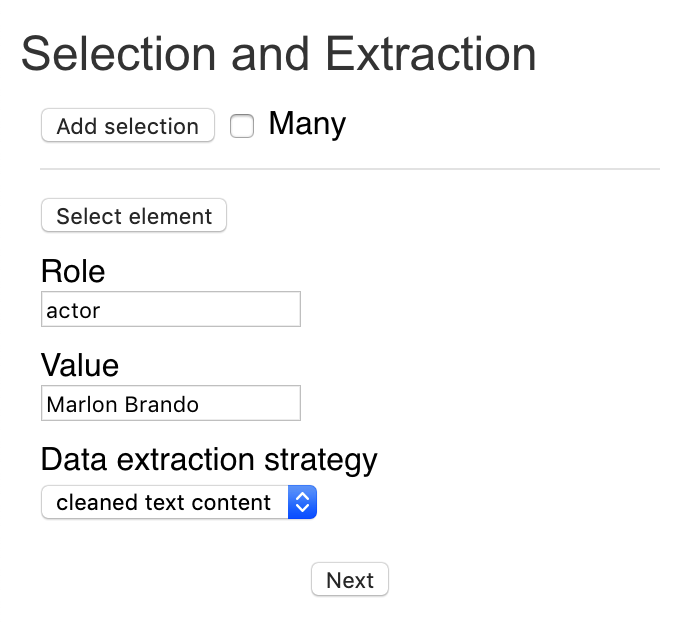
\includegraphics[width=0.80\linewidth]{tool/sel.png}}
%     \caption{Selection and Extraction}
%     \label{fig-selectionExtraction}
% \end{figure}



\subsection{Querying}

% \begin{figure}
%   \centering
%     \fbox{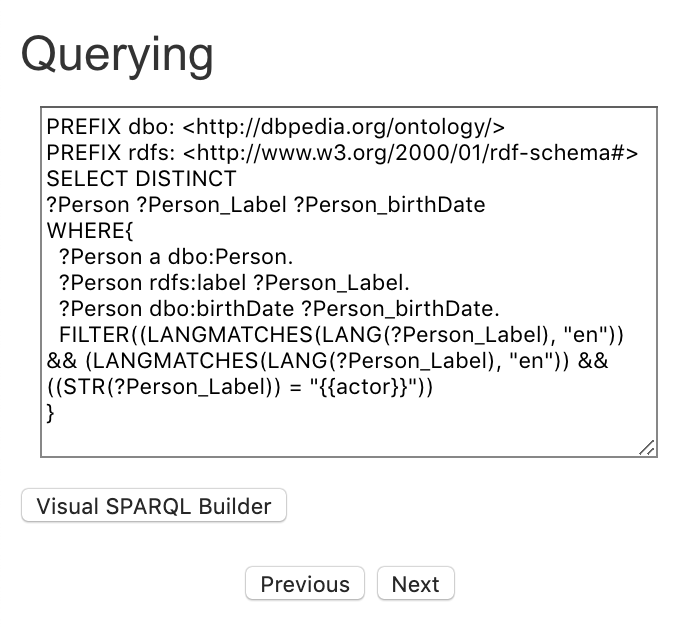
\includegraphics[width=0.80\linewidth]{tool/2_que_cut.png}}
%     \caption{Querying}
%     \label{fig-querying}
% \end{figure}

Once the Selection and Extraction stage is done, the semantic query that will retrieve the new information from the SW must be defined. There are different mechanisms to help the SPARQL query building with visual tools such as ExConQuer \cite{Attard2017ExConQuerRe-use} or Visual SPARQL Builder (VSB) \cite{mci/Eipert2015}. In our approach, we delegate the SPARQL query building to VSB, which provides an intuitive interface to assist users in vocabulary and properties detection.
The tool provides a text input field for the query, with a link to the VSB Web application, where the user should build the query and then send it back to the input field. VSB has also been augmented for better integration with the tool. The resulting SPARQL query will be executed against the DBpedia SPARQL endpoint, obtaining the augmentation data.

\subsection{Building}


% \begin{figure}
%   \centering
%     \fbox{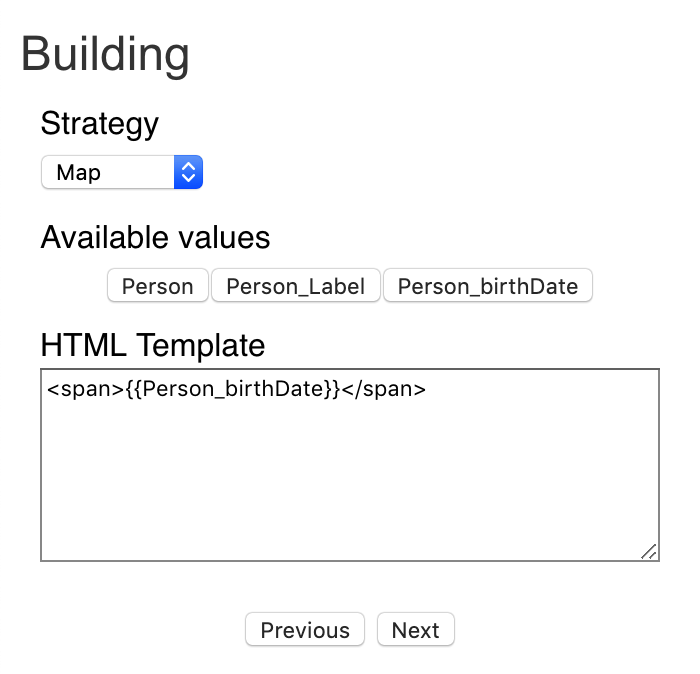
\includegraphics[width=0.80\linewidth]{tool/3_bui_cut.png}}
%     \caption{Building}
%     \label{fig-building}
% \end{figure}


This step involves the definition of the HTML template that will be used to insert the augmentation data to the Web page. The user must write the HTML code including references to the augmentation data; however, the template may consist of only references, thus not being mandatory for the user to know any HTML. References to augmentation data are presented as buttons that, when clicked, are inserted into the text input for the template.

\subsection{Insertion}

This step configures the weaving of the HTML augmentation elements built in the previous step. The user must choose the wanted places in the Web page to inject them. This is done similarly to the Selection step, by selecting HTML elements from the DOM.

% \begin{figure}
%   \centering
%     \fbox{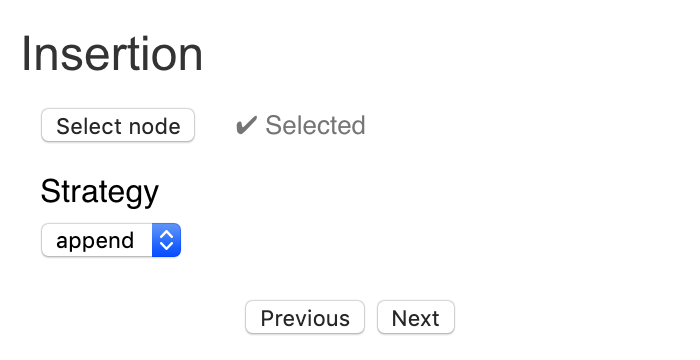
\includegraphics[width=0.80\linewidth]{tool/4_ins_cut.png}}
%     \caption{Insertion}
%     \label{fig-insertion}
% \end{figure}


\subsection{Saving}

% \begin{figure}
%   \centering
%     \fbox{
\includegraphics[width=0.80\linewidth]{tool/5_sav_cut.png}}
%     \caption{Saving}
%     \label{fig-saving}
% \end{figure}


The user will define a set of URLs where the augmentation should be applied. In our cast example, this would be \texttt{https://www.imdb.com/title/*}. The tool now shows two buttons: \textit{save}, which saves the augmentation script to apply it every time the user opens a website that match the specified expression; and \textit{try}, which performs the augmentation, letting the user see the changes that the augmentation produce in the Web page. Figure \ref{fig-oscars} shows the cast section of the \textit{``The Godfather''} page before and after the augmentation.



% \section{Case Studies}
% \label{sec-casestudies}

% This section introduces two examples of the utilization of the proposed approach to augment Web pages with the use of SW content. Both examples use DBpedia as the SW representation because it is the most important node in the LOD cloud\cite{DBpediaJournal}. 

% \subsection{The Oscars augmentation for cast lists in IMDb}
% \label{sec-imdb}


\begin{figure}
  \centering
    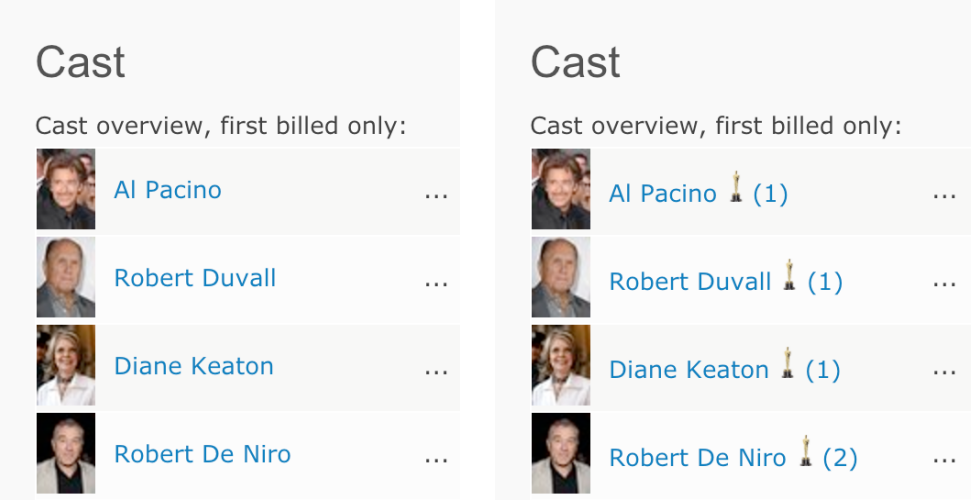
\includegraphics[width=0.7\linewidth]{oscars6.png}
    \caption{Case study: Oscars}
    \label{fig-oscars}
\end{figure}

% The goal of this augmentation is to add the number of Oscars that each cast member in an IMDb page has won (not necessarily within the film). First, each actor's and actress' names are extracted from the DOM. Then, the amount of won Oscars is collected via a SPARQL query (a simplified version of this query for Al Pacino is shown in Listing \ref{l-oscars}), and the HTML template for adding the information to the website is defined (\ref{l-oscars_template}). On the left side of Figure \ref{fig-oscars} the cast list for The Godfather II is shown as appears in IMDb; on the right side, the cast list is shown after the augmentation has been executed. It has been added, besides the name of every actor, an academy award image and the number of Oscars s/he won. 


\section{Related Work}
\label{sec-related_work}
In the literature there are several references regarding the use of SW either to improve user experience, to help client-side developers to manipulate semantic data or to \textit{semantify} non-semantic pages. 
Rico et al. \cite{Rico2012AData} introduced a tool to allow Web developers with no knowledge about SW technologies to create Web templates capable of handling semantic data. 
The Pundit \cite{Grassi2013Pundit:Semantics} tool provides a set of libraries to annotate content with semantic information and complement it with information generated by a SPARQL query. 
Orabona et al. \cite{Orabona2015AnPortals.} proposed the use of SW to enhance content management systems with the use of a triplet store, on the server side. 
WOA \cite{DBLP:conf/icwe/FirmenichBRWB16} presents an approach for the creation of WA layers by firstly annotating Web contents with semantic tags. 
However, for the best of our knowledge, there exists no end-user programming tools for defining the weaving of information extracted from the SW in the current context of Web browsing.
 
\section{Conclusions and Further Work}
\label{sec-conclusions}

%The SW is in a mature state since many years. However, it is not common to see tools for allowing Web users communities to consume all this infrastructure. In this paper, we present a SWA framework called \SWAT, which helps \textit{userscripters} without SW knowledge to develop \textit{userscripts} oriented to Web sites contents. The Framework was instantiated for multiple examples showing the feasibility of our approach. Currently, we are designing and developing the end-User development tool, which aims to reach not only \textit{userscripters}, but also end-users with none programming skills. Future works include an evaluation with developers (for the use of the framework), and with end-users (for the tool shown in Section 5).

The SW is in a mature state since many years. However, it is not common to see tools for allowing Web users communities to consume all this infrastructure. In this paper, we present a pipeline processs for building SWA, and an End-User Development tool based upon it called SWAX to create augmentation layers. The approach allows end-users without any programming skills to produce generic WA scripts that allow for enriching the contents of groups of Web pages.

The first future work is the need for an exhaustive evaluation. The prominent prototype demonstrated well behavior, and easy to use augmentation tasks in laboratory tests. Nonetheless, we are designing usability tests with a group of developers. Additionally, more extraction and insertion strategies are in development, as well as user experience improvements. The current version of the SWAX works with VSB, but there are several SPARQL query builders that could be adapted for SWAX.


%
% ---- Bibliography ----
%
% BibTeX users should specify bibliography style 'splncs04'.
% References will then be sorted and formatted in the correct style.
%
% \bibliographystyle{splncs04}
% \bibliography{mybibliography}
%
\bibliographystyle{splncs04}
\bibliography{biblio}
\end{document}
